\documentclass[letterpaper,12pt,fleqn]{article}
\usepackage{matharticle}
\usepackage{tikz}
\usepackage{forloop}
\pagestyle{empty}
\newcommand{\e}{\epsilon}
\begin{document}
\section*{Regions}

\begin{definition}
  A \emph{neighborhood} of $z_0\in\C$ is the locus given by:
  \[\abs{z-z_0}<\e\]
  For some $\e>0$.

  \begin{figure}[h]
    \setlength{\leftskip}{1in}
    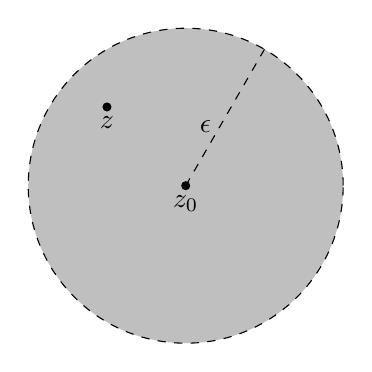
\begin{tikzpicture}
      \draw [dashed,fill=lightgray] (0,0) circle [radius=2];
      \draw [fill=black] (0,0) circle [radius=0.05];
      \draw [fill=black] (-1,1) circle [radius=0.05];
      \draw [dashed] (0,0) -- (1,1.732);
      \node [below] at (0,0) {$z_0$};
      \node [below] at (-1,1) {$z$};
      \node at (0.25,0.75) {$\e$};
    \end{tikzpicture}
  \end{figure}
\end{definition}

\begin{definition}
  A \emph{deleted neighborhood} of $z_0\in\C$ is the locus given by:
  \[0<\abs{z-z_0}<\e\]
  For some $\e>0$.

  \begin{figure}[h]
    \setlength{\leftskip}{1in}
    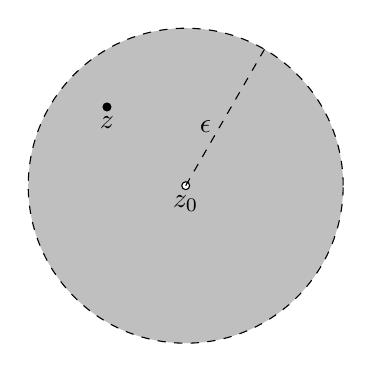
\begin{tikzpicture}
      \draw [dashed,fill=lightgray] (0,0) circle [radius=2];
      \draw [fill=white] (0,0) circle [radius=0.05];
      \draw [fill=black] (-1,1) circle [radius=0.05];
      \draw [dashed] (0,0) -- (1,1.732);
      \node [below] at (0,0) {$z_0$};
      \node [below] at (-1,1) {$z$};
      \node at (0.25,0.75) {$\e$};
    \end{tikzpicture}
  \end{figure}
\end{definition}

\begin{definition}
  Let $S\subseteq\C$:
  \begin{itemize}
  \item To say that $z_0\in\C$ is an \emph{interior point} of $S$ means that
    there exists a neighborhood $N$ of $z_0$ such that $N\subseteq S$.

  \item To say that $z_0\in\C$ is an \emph{exterior point} of $S$ means that
    there exists a neighborhood $N$ of $z_0$ such that $N\cap S=\emptyset$.

  \item To say that $z_0\in\C$ is a \emph{boundary point} of $S$ means that
    for all neighborhoods $N$ of $z_0, N$ contains both interior and exterior
    points:
    \[N\cap S\ne\emptyset$ and $N-S\ne\emptyset\]
  \end{itemize}
\newpage
  \begin{figure}[h]
    \setlength{\leftskip}{1in}
    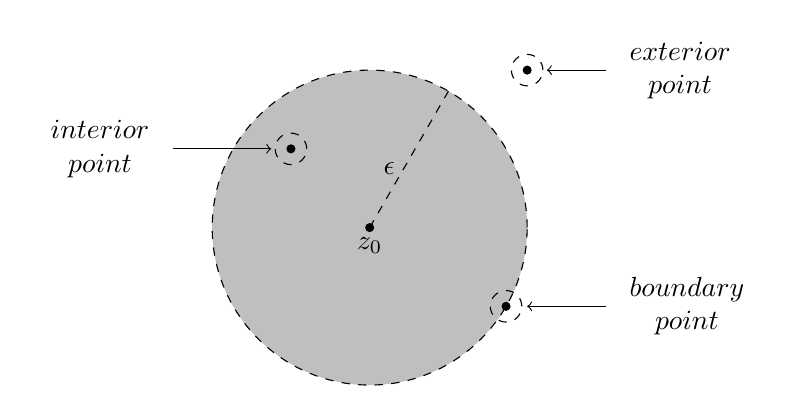
\begin{tikzpicture}
      \draw [dashed,fill=lightgray] (0,0) circle [radius=2];
      \draw [fill=black] (0,0) circle [radius=0.05];
      \draw [dashed] (0,0) -- (1,1.732);
      \node [below] at (0,0) {$z_0$};
      \node at (0.25,0.75) {$\e$};
      \draw [fill=black] (-1,1) circle [radius=0.05];
      \draw [dashed] (-1,1) circle [radius=0.2];
      \draw [fill=black] (2,2) circle [radius=0.05];
      \draw [dashed] (2,2) circle [radius=0.2];
      \draw [fill=black] (1.732,-1) circle [radius=0.05];
      \draw [dashed] (1.732,-1) circle [radius=0.2];
      \draw [->] (3,2) -- (2.25,2);
      \draw [->] (-2.5,1) -- (-1.25,1);
      \draw [->] (3,-1) -- (2,-1);
      \node [right] at (3,2) {$\begin{array}{c}exterior\\point\end{array}$};
      \node [left] at (-2.5,1) {$\begin{array}{c}interior\\point\end{array}$};
      \node [right] at (3,-1) {$\begin{array}{c}boundary\\point\end{array}$};
    \end{tikzpicture}
  \end{figure}
\end{definition}

Given a set $S\subseteq\C$, a point $z_0\in\C$ is either an interior, exterior,
or boundary point for $S$.

\begin{definition}
  Let $S\subseteq\C$. The \emph{boundary} of $S$ is the set:
  \[B=\{b\in\C\mid b\ \mbox{is a boundary point for}\ S\}\]
\end{definition}

\begin{definition}
  Let $S\subseteq\C$ with boundary $B$:
  \begin{itemize}
  \item To say that $S$ is \emph{open} means $S\cap B=\emptyset$.
  \item To say that $S$ is \emph{closed} means $B\subseteq S$.
  \item To say that $S$ is \emph{clopen} means that $S$ is both open and
    closed.
  \item The \emph{closure} of $S$ is given by:
    \[\bar{S}=S\cup B\]
  \end{itemize}
\end{definition}

\begin{example}
  \[S=\left\{\frac{1}{n}\mid n\in\N\right\}\]

  \bigskip
  
  \begin{minipage}{3in}
    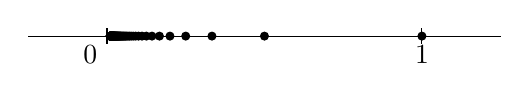
\begin{tikzpicture}
      \draw (-1,0) -- (5,0);
      \draw (0,0.1) -- (0,-0.1);
      \draw (4,0.1) -- (4,-0.1);
      \newcounter{loop}
      \forloop{loop}{1}{\value{loop}<100}{
        \draw [fill=black] ({4/\value{loop}},0) circle [radius=0.05];
      }
      \node [below left] at (0,0) {$0$};
      \node [below] at (4,0) {$1$};
    \end{tikzpicture}
  \end{minipage}
  \begin{minipage}{3in}
    $S$ contains no interior points; they are all boundary points.
  \end{minipage}
\end{example}

\begin{example}
  $\C$ is clopen, since $B=\emptyset$:
  \[\C\cap B=\C\cap\emptyset=\emptyset\]
  \[B=\emptyset\subset\C\]
\end{example}

\begin{example}
  The punctured disk $0<\abs{z-z_0}\le\e$ is neither open nor closed; it
  contains the boundary points on the circle; however, it does not include the
  boundary point at the excluded center.
\end{example}

\begin{definition}
  To say that a set $S\subseteq\C$ is connected means:
  \begin{enumerate}
  \item $S$ is open.
  \item $\forall\,z_1,z_2\in S,$ there exists a path that connects the two
    points consisting of a finite number of line segments
    $L=\bigcup_{k=1}^n\ell_k$ such that $L\subseteq S$.
  \end{enumerate}
\end{definition}

\begin{example}
  Consider the (open) annulus $a\le\abs{z-z_0}\le b$:

  \bigskip
  
  \begin{figure}[h]
    \setlength{\leftskip}{1in}
    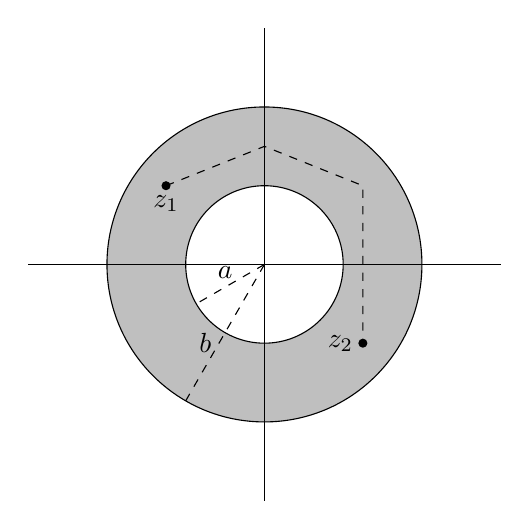
\begin{tikzpicture}
      \draw [fill=lightgray] (0,0) circle [radius=2];
      \draw [fill=white] (0,0) circle [radius=1];
      \draw [fill=black] (-1.25,1) circle [radius=0.05];
      \draw [fill=black] (1.25,-1) circle [radius=0.05];
      \draw [dashed] (-1.25,1) -- (0,1.5) -- (1.25,1) -- (1.25,-1);
      \node [below] at (-1.25,1) {$z_1$};
      \node [left] at (1.25,-1) {$z_2$};
      \draw (-3,0) -- (3,0);
      \draw (0,-3) -- (0,3);
      \draw [dashed] (0,0) -- (-0.866,-0.5);
      \draw [dashed] (0,0) -- (-1,-1.732);
      \node at (-0.5,-0.1) {$a$};
      \node at (-0.75,-1) {$b$};
    \end{tikzpicture}
  \end{figure}
\end{example}

\begin{definition}
  Let $S\subseteq C$. To say that $S$ is a \emph{domain} means:
  \begin{enumerate}
  \item $S\ne\emptyset$
  \item $S$ is open
  \item $S$ is connected
  \end{enumerate}

  A set consisting of a domain and zero or more of its boundary points is
  called a \emph{region}.
\end{definition}

\begin{definition}
  Let $S\subseteq\C$. To say that $S$ is bounded means:
  \[\exists\,r\in\R\mid\forall\,z\in S,\abs{z}\le r\]
\end{definition}
\newpage
\begin{definition}
  Let $S\subseteq C$. To say that $z_0\in S$ is an accumulation (limit) point
  of $S$ means for all deleted neighborhoods $N$ of $z_0, N\cap S\ne\emptyset$.
\end{definition}

\begin{example}
  \[S=\left\{\frac{i}{n}\mid n\in\N\right\}\]

  \bigskip
  
  \begin{minipage}{3in}
    \begin{tikzpicture}
      \draw (-3,0) -- (3,0);
      \draw (0,-1) -- (0,5);
      \draw (-0.1,2) -- (0.1,2);
      \draw (-0.1,4) -- (0.1,4);
      \forloop{loop}{1}{\value{loop}<100}{
        \draw [fill=black] (0,{4/\value{loop}}) circle [radius=0.05];
      }
      \draw [dashed] (0,2) circle [radius=0.2];
      \node [below left] at (0,0) {$0$};
      \node [left] at (0,4) {$i$};
      \node [left] at (0,2) {$\frac{i}{2}$};
    \end{tikzpicture}
  \end{minipage}
  \begin{minipage}{3in}
    $\frac{i}{2}$ is not a limit point for $S$. In fact, the only limit point
    for $S$ is $0$.
  \end{minipage}
\end{example}
    
\end{document}
